\documentclass{article}
\usepackage[margin=2cm]{geometry}
\usepackage{graphicx}
\usepackage[pages=some]{background}
\usepackage{titling}
\usepackage{tabularx}
\usepackage{tikz}
\usepackage{enumitem}
\usepackage{amsmath}
\usepackage{amssymb}
\usepackage{tcolorbox}
\usepackage{subcaption}
\usepackage{multicol}
\usepackage{float}

\geometry{a4paper}

\backgroundsetup{
    scale=1,
    angle=0,
    opacity=1,
    contents={%
        
\includegraphics[width=\paperwidth,height=\paperheight]{institution_logo.jpg}
    }
}

\newcommand{\subtitle}[1]{
    \posttitle{
        \par\end{center}
        \begin{center}\large#1\end{center}
        \vskip0.5em}
}

\title{IPE-431}
\author{Md. Hasibul Islam}
\subtitle{MACHINE TOOLS}

\begin{document}
\begin{titlepage}
    \centering
    
    {\Huge\bfseries\maketitle}
    \textbf{Sristy Mam} \\
    \vspace{2cm}
    
\includegraphics[width=8cm]{institution_logo.jpg}
    \vfill
    \vspace*{2cm}
\end{titlepage}

\tableofcontents
\pagebreak
\section{Lecture 01: Introduction} 
\hfill Date: 06/06/2023
\begin{itemize}
  \item \textbf{Conventional Machining}: Conventional machining refers to traditional manufacturing processes that involve the removal of material from a workpiece to achieve the desired shape or form. These processes typically utilize cutting tools such as drills, lathes, milling machines, or grinding machines to remove material through cutting, grinding, drilling, or similar operations. Conventional machining techniques are well-established and widely used in industries for shaping and finishing operations.

\item \textbf{Non-conventional Machining}: Non-conventional machining, also known as unconventional or advanced machining, encompasses a set of manufacturing processes that do not rely on traditional cutting tools. These processes use various methods to shape or modify materials, often involving thermal, chemical, electrical, or mechanical energy. Examples of non-conventional machining include electrical discharge machining (EDM), laser cutting, waterjet cutting, electrochemical machining (ECM), ultrasonic machining (USM), and abrasive jet machining (AJM). These techniques are particularly useful for materials that are difficult to machine using conventional methods or when intricate or complex shapes are required.

\item \textbf{Subtractive Manufacturing}: Subtractive manufacturing, also known as subtractive processes, refers to the manufacturing methods that involve the removal of material from a larger block or workpiece to create the desired shape or form. Conventional machining processes fall under the category of subtractive manufacturing. These processes selectively remove material until the final shape or dimensions are achieved. Subtractive manufacturing is commonly used in industries such as metalworking, woodworking, and plastics manufacturing, where excess material is removed to create the desired end product.

\item \textbf{Additive Manufacturing}: Additive manufacturing, also referred to as 3D printing, is a revolutionary manufacturing approach that involves the creation of three-dimensional objects by adding material layer by layer. In additive manufacturing, a digital model or design is converted into a physical object by adding successive layers of material, typically through processes like fused deposition modeling (FDM), stereolithography (SLA), selective laser sintering (SLS), or binder jetting. Additive manufacturing offers design freedom, customization, rapid prototyping, and the ability to produce complex geometries that are challenging or impossible to achieve with traditional manufacturing methods. It has found applications in various industries, including aerospace, automotive, medical, and product development. 
\end{itemize}


\subsubsection*{Books List}
\begin{itemize}
  \item Machine tools \hfill by Charnov
  \item Elements of Machines \hfill by Anwarul Azim 
\end{itemize}
\newpage

\section{Lecture 2: Types of Machine Tools}
\hfill Date: 13/06/2023
\subsubsection*{Uses of Tailstock:}
The term "tailstock" refers to a component found in many machine tools, such as lathes and milling machines. It serves several important purposes:
\begin{enumerate}
  \item Support: The tailstock provides support and stability to the workpiece being machined. It acts as a counterpoint to the cutting forces exerted by the tool, ensuring accurate and controlled machining.
  \item Centering: In turning operations, the tailstock contains a rotating center (known as a live center) that aligns with the workpiece's center. This helps in achieving concentricity and accurate turning operations.
  \item Drilling: The tailstock can be used for drilling operations by mounting a drill chuck or drill bit onto its quill. This allows for precise and controlled drilling operations on the workpiece.
  \item Boring: By attaching a boring bar to the tailstock, it is possible to perform accurate and controlled boring operations on the workpiece. Boring involves enlarging existing holes or creating cylindrical recesses with tight tolerances.Taper turning: Some tailstocks can be adjusted to a specific angle, allowing for taper turning operations. This is useful when creating tapered features, such as conical shapes or tapered shafts.
\end{enumerate}

\subsubsection*{Types of chips:}
There are several types of chips that can occur during machining processes. The type of chip formed depends on various factors, including the material being machined, the cutting tool geometry, cutting speed, feed rate, and depth of cut. Here are some common types of chips and the materials in which they typically occur:

\begin{enumerate}
  \item Continuous Chip: Continuous chips are long, continuous curls of material. They occur primarily in \textbf{ductile materials such as aluminum, copper, mild steel, and stainless steel}. These materials have high ductility, which allows the material to deform plastically and form continuous chips.
  \item Discontinuous Chip: Discontinuous chips are short, broken chips that are typically formed in \textbf{brittle materials such as cast iron and some types of hardened steels}. These materials have low ductility, which causes the chips to break and form shorter segments.
  \item Built-Up Edge (BUE): A built-up edge is a localized region of material that adheres to the cutting tool edge during machining. It occurs in materials like \textbf{low carbon steels and alloys containing high carbon content}. The BUE can affect the chip formation and lead to variations in chip type.
  \item Serrated Chip: Serrated chips have a wavy or sawtooth-like appearance. They occur in materials like\textbf{ titanium and some high-temperature alloys}. These materials have low thermal conductivity, which causes the heat generated during cutting to be concentrated in narrow bands, resulting in the formation of serrated chips.
\end{enumerate}

\subsubsection*{Why discontinuous chips are better than continuous chips:}
\begin{enumerate}
  \item Improved chip disposal: Discontinuous chips are shorter and easier to evacuate from the machining zone, reducing the risk of chip entanglement, jamming, and workpiece/tool damage.
  \item Reduced heat generation: Discontinuous chips allow for better heat dissipation, preventing excessive heat buildup that can lead to tool wear, workpiece deformation, and poor surface finish.
  \item Lower cutting forces: Discontinuous chips require less cutting force, resulting in reduced power consumption, minimized tool deflection, and improved machining stability.
  \item Enhanced surface finish: Discontinuous chips reduce the occurrence of issues like built-up edge, poor surface finish, and material smearing, leading to improved surface quality.
  \item Reduced workpiece deformation: Discontinuous chips distribute cutting forces more evenly, minimizing the risk of workpiece distortion or inaccuracies in the machined part.
\end{enumerate}

\subsubsection*{Chip breaker \& it's use:}
A chip breaker is a feature in cutting tools that helps control chip formation during machining. Its uses include:
\begin{itemize}
  \item Chip control: Breaking long chips into shorter segments or controlled shapes.
  \item Preventing chip clogging: Ensuring effective chip evacuation from the cutting zone.
  \item Tool life improvement: Reducing chip-related issues and tool damage.
  \item Surface finish enhancement: Minimizing vibrations and irregularities for a smoother finish.
  \item Material-specific design: Tailoring chip breakers to different materials and operations.
\end{itemize}

\subsection*{Types of machine tools}
\begin{enumerate}
  \item According to size:
    \begin{enumerate}
      \item Light duty :  Smaller, less powerful machines for small-scale or hobbyist applications and light machining tasks. 
      \item Medium duty : Sturdier machines with higher power for workshops and small to medium-sized production operations
      \item Heavy duty:  Robust, powerful machines for demanding industrial applications, large-scale production, and heavy machining tasks.
    \end{enumerate}
  \item According to the method of actuation 
    \begin{enumerate}
      \item Manually 
      \item Semi-automatic 
      \item Automated
    \end{enumerate}
  \item According to the purposes 
    \begin{enumerate}
      \item General Purposes : Versatile machines for a wide range of machining tasks. Ex - Lathe machine 
      \item Special Purposes : Designed for specific applications with customized features and higher efficiency. Ex - Gear hobbing machine 
    \end{enumerate}
  \item According to rotation 
    \begin{enumerate}
      \item Rotary cutting machine : Lathe machine, Drilling machine 
      \item Linear cutting machine : Shaper machine, Planner machine 
    \end{enumerate}
  \item According to feed  
    \begin{enumerate}
      \item Axial Feed : Axial feed refers to the movement of the cutting tool or workpiece along the axis of rotation or the longitudinal direction. It involves the tool or workpiece moving in a straight line parallel to the axis of rotation. In turning operations on a lathe, the axial feed corresponds to the tool advancing or retracting along the workpiece's length.
      \item Transverse Feed : Transverse feed refers to the movement of the cutting tool or workpiece perpendicular to the axis of rotation. It involves the tool or workpiece moving in a direction that is perpendicular to the axis of rotation. In milling operations, the transverse feed corresponds to the lateral movement of the cutting tool as it removes material from the workpiece.
    \end{enumerate}
\end{enumerate}

\subsubsection*{Why turning is called micro-threading:}
While threading, we use higher feed rate. when feed rate becomes less, the threading becomes denser. For turning, the feed rate is very low, that's why no visible threads are perceived and creates a smooth surface. That's why, turning is called micro-threading. 

\subsection*{Gear Mathmatical Relations:}
\begin{figure*}
  \centering
  \includegraphics*[width=0.7\textwidth]{img/gear_nomen.png}
  \caption{Gear Nomenclature}
\end{figure*}

\begin{align*}
  v &\Rightarrow \text{volume} &
  b &\Rightarrow \text{face width} &
  d &\Rightarrow \text{diameter of pitch circle} \\
  m &\Rightarrow \text{module of gear} & 
  t &\Rightarrow \text{No of teeth} &
  M &\Rightarrow \text{Mass of gear} \\ 
  n &\Rightarrow \text{Rotation in RPM} & 
  \omega &\Rightarrow \text{angular velocity} &
  \rho &\Rightarrow \text{Density of Gear materials} \\ 
  I &\Rightarrow \text{Moment of Inertia} & 
  F &\Rightarrow \text{Force} &
  T &\Rightarrow \text{Torque} \\
  P &\Rightarrow \text{Total power} &
  KE &\Rightarrow \text{Kinetic Energy} & 
  \text{m'} &\Rightarrow \text{Addendtum \& Dedendum} 
\end{align*}



\begin{tabularx}{\textwidth}{X|X|X}
  \centering 
  \begin{align*}
    v = \frac{\pi}{4} d^2 b \\ 
    v \propto bd^2 \\
     \\
    F \propto A  \left[\text{Surface area}\right]\\
    v \propto (m'+m')b \\
    v \propto m'b \\
    \\
    T \propto Fd \\
    T \propto m'bd\\
  \end{align*} & 
  \begin{align*}
    P \propto T \omega\\
    P \propto m'bdn \\
    \\
    KE = \frac{1}{2} I \omega^2 \\
    KE = \frac{1}{2} \frac{Md^2}{8} \left(\frac{2\pi n}{60}\right)^2\\
    KE \propto Md^2n^2 \\
    \propto \rho V d^2 n^2 \\
    \propto \rho b d^4 n^2 
  \end{align*} &
  \begin{align*}
    \propto \rho \left(m'bdn\right) \frac{d^3n}{m'} \\
    \propto \rho P \frac{d^3 n}{m'}\\
    \text{If } \rho \text{ and P are kept constant,}\\
    \propto \frac{d^3 n}{m} \\
    \propto \frac{d^2\left(mT\right)n}{m} \\
    \propto d^2 T n 
  \end{align*} 
\end{tabularx}

\subsubsection*{Requirements of Machine Tools:}
A good machine tool should have:
\begin{itemize}
  \item \textbf{Accuracy}: High precision and accuracy in machining operations.
  \item \textbf{Rigidity}: Structural stability to withstand cutting forces and vibrations.
  \item \textbf{Power and Speed}: Adequate power and speed for efficient machining.
  \item \textbf{Versatility}: Ability to handle various machining operations and workpiece materials.
  \item \textbf{Ease of Use}: User-friendly features and ergonomic design.
  \item \textbf{Reliability and Durability}: Consistent performance and long-term durability.
  \item \textbf{Safety Features}: Incorporation of safety measures for operator protection.
  \item \textbf{Cost-effectiveness}: Value for money in terms of cost, maintenance, and productivity.
  \item \textbf{Service and Support}: Availability of technical support and maintenance services.
  \item \textbf{Adaptability}: Potential for upgrades and compatibility with emerging technologies.
\end{itemize}

\subsubsection*{Breakdown Frequency}
Breakdown frequency in a machine tool refers to the rate of failures or malfunctions that require repair or maintenance. It varies based on factors like machine quality, design, maintenance, and usage. Lower breakdown frequency improves productivity, while higher frequency leads to more interruptions and reduced efficiency. Proper maintenance and using reliable machine tools help reduce breakdown frequency and minimize costs associated with repairs and downtime. Tracking breakdown frequency aids in identifying recurring issues and optimizing machine performance.

\subsubsection*{How Productivity can be maximized:}
\begin{enumerate}
  \item Efficient Workflow: Designing an optimized workflow ensures smooth material flow, minimizes idle time, and reduces non-value-added activities. Analyze and streamline processes to eliminate bottlenecks and optimize the sequence of operations.

\item Cutting Parameters Optimization: Fine-tuning cutting parameters such as cutting speed, feed rate, and depth of cut can significantly impact productivity. Balancing these parameters to achieve the optimal balance between material removal rate and tool life can improve efficiency.

\item Tooling Selection and Maintenance: Selecting the right cutting tools based on the material, operation, and desired outcome is crucial. Additionally, proper tool maintenance, including regular sharpening/replacement, ensures optimal cutting performance and minimizes downtime.

\item Automation and CNC: Incorporating automation, robotics, and computer numerical control (CNC) systems reduces manual intervention, enhances precision, and speeds up operations. Automation can be employed for material handling, tool changing, and repetitive tasks, freeing up operators for more complex operations.

\item Workpiece and Fixture Design: Well-designed workpieces and fixtures facilitate faster setup times, ease of clamping, and improved access for cutting tools. Ensuring proper workpiece stability and accurate positioning can reduce setup and changeover times.

\item Continuous Monitoring and Control: Implementing real-time monitoring systems allows for proactive detection of abnormalities, tool wear, and machine performance issues. By identifying potential problems early on, corrective actions can be taken promptly, minimizing unplanned downtime.

\item Operator Training and Skill Development: Providing comprehensive training to machine operators enhances their proficiency in machine operations, tooling changes, and troubleshooting. Skilled operators can optimize machine utilization, minimize errors, and perform timely maintenance.

\item Lean Manufacturing Principles: Adopting lean manufacturing principles, such as 5S, visual management, and waste reduction techniques, promotes a more efficient and organized work environment. Eliminating non-value-added activities and optimizing processes improves overall productivity.

\item Data-driven Decision Making: Utilizing data analytics and performance metrics helps identify areas for improvement, track key performance indicators (KPIs), and make informed decisions. Data analysis can highlight opportunities to optimize processes, reduce cycle times, and increase throughput.

\item Continuous Improvement Culture: Foster a culture of continuous improvement by encouraging feedback, suggestions, and involvement from operators and technicians. Regularly evaluate processes, identify improvement opportunities, and implement changes based on lessons learned.
\end{enumerate}

\subsubsection*{Precision of Machine tools depends upon:}
\begin{enumerate}
  \item Machine Design and Construction: The design and construction of the machine tool play a significant role in its precision. A rigid and stable structure with proper alignment and precision components is essential for maintaining accuracy during machining operations.

  \item Control System: The control system, such as computer numerical control (CNC), influences precision by accurately interpreting and executing machining instructions. A high-quality control system with advanced algorithms and precise positioning capabilities enhances the precision of the machine tool.
  
  \item Mechanical Components: The quality and precision of mechanical components, such as spindles, guideways, bearings, and screws, directly affect the precision of the machine tool. High-quality components with tight tolerances and minimal backlash contribute to improved precision.
  
  \item Cutting Tools: The selection and condition of cutting tools impact precision. High-quality tools with proper geometry, sharp edges, and accurate dimensions ensure precise cutting and dimensional accuracy.
  
  \item Metrology and Calibration: Regular calibration and maintenance of the machine tool using metrology equipment, such as precision measuring instruments and laser alignment systems, help maintain accuracy over time. Accurate calibration ensures that the machine tool performs as intended and delivers precise results.
  
  \item Environmental Factors: External factors like temperature, humidity, and vibrations can affect the precision of machine tools. Controlling the environmental conditions within acceptable limits helps maintain stability and accuracy during machining operations.
  
  \item Operator Skill and Training: The skill and expertise of the operator influence the precision of the machine tool. Proper training on machine operation, tool setup, and measurement techniques helps operators understand and implement precise machining practices.
  
  \item Process Planning and Parameters: The selection and optimization of cutting parameters, tool paths, and machining strategies impact precision. Proper process planning and parameter selection considering the material, tooling, and desired tolerances contribute to achieving the desired precision.
\end{enumerate}

\section{Lecture 03: Regulation of speed \& Feed rate} 
\hfill Date: 19/06/2023 \\

The optimum and most economical speeds for the two machining
movements—the cutting and the feed movement are determined by-
• tool materials and workpiece materials
• tool shape
• type of machining processes
• required surface quality

\subsection*{Machining Cost}
A machining operation should be conducted at such values of cutting
parameters (speed, feed, depth of cut etc.) that ensure the minimum
cost price of the machined component.\\
The machining cost can be expressed by the equation - 
$$C = C_{mt} + C_{npt} + C_{tc} + C_t$$
here,\\ 
$C =$ machining cost \\
$C_{mt} =$ the cost of machining time \\
$C_{npt} =$ the cost of non-productive time; such as loading and unloading, idle travel of cutting tool. \\
$C_{tc} =$ tool changing cost per component \\
$C_{t} =$ the cost of the tool per component \\

\begin{figure}[h]
  \begin{center}
    \includegraphics*[width=0.8\linewidth]{img/cost_func.jpeg}
    \caption{Machining cost graph}
  \end{center}
\end{figure}

\subsection*{Some Important Mathematical Expression}
Taylor's tool life formula: 
$$VT^n = C$$
here, V = cutting velocity, T = cutting time, n = tool life index, C = constant.\\
cutting velocity formula: 
$$V = \frac{\pi n d}{1000} \, m/min$$
here, \\
n = rotation in rpm, d = diameter of rotating workpiece (in mm)\\
$$\Rightarrow n \propto \frac{1}{d}$$
so, we get, 
$$n_{min} = \frac{V_{max} \times 1000}{\pi \times d_{min}}$$
$$n_{max} = \frac{V_{min} \times 1000}{\pi \times d_{max}}$$

The speed range ratio ,
\begin{align*}
  R_n &= \dfrac{n_{max}}{n_{min}}\\
  &= \frac{v_{max}}{v_{min}} \frac{d_{max}}{d_{min}} \\
  &= R_v \times R_d
\end{align*}
Here, $R_v$ = cutting speed range ratio, $R_d$ = diameter range ratio.\\
Point : $\checkmark V_{min} \rightarrow d_{min}\, \& \, V_{max} \rightarrow d_{max}$   


\textbullet In shaper machine, $R_n = R_v$. Because, there is no effect of diameter in case of shaping. 

\subsection*{Law of stepped revolution}
\subsubsection*{Geometric Progression}
\begin{align*}
  n_1 \\
  n_2 &= n_1 \phi \\
  n_3 &= n_2 \phi &= n_1 \phi^2\\ 
  n_4 &= n_3 \phi &= n_1 \phi^3\\
  .\\
  .\\
  n_z &= n_{z-1} \phi &= n_1 \phi^{z-1}\\
\end{align*}
here, $\phi$ = prograssive ratio (a constant) \\
so, we get, $$\phi = \left(\frac{n_z}{n_1}\right)^{\frac{1}{z-1}}$$

\subsubsection*{Example}
Calculate the rpm values and diameter range served by each rpm for
the following conditions:\\
$n_1$ = 30 rpm,
$n_z$ = 375 rpm,
Number of speed steps, z = 12,
v = 20 m/min, Assume, initial diameter = 212 mm.

\textbf{Solution:}\\
$$\phi = \left(\frac{375}{30}\right)^{\frac{1}{12-1}} = 1.26$$

\begin{figure}[h]
  \centering

  \begin{subfigure}{0.48\textwidth}
    \centering
    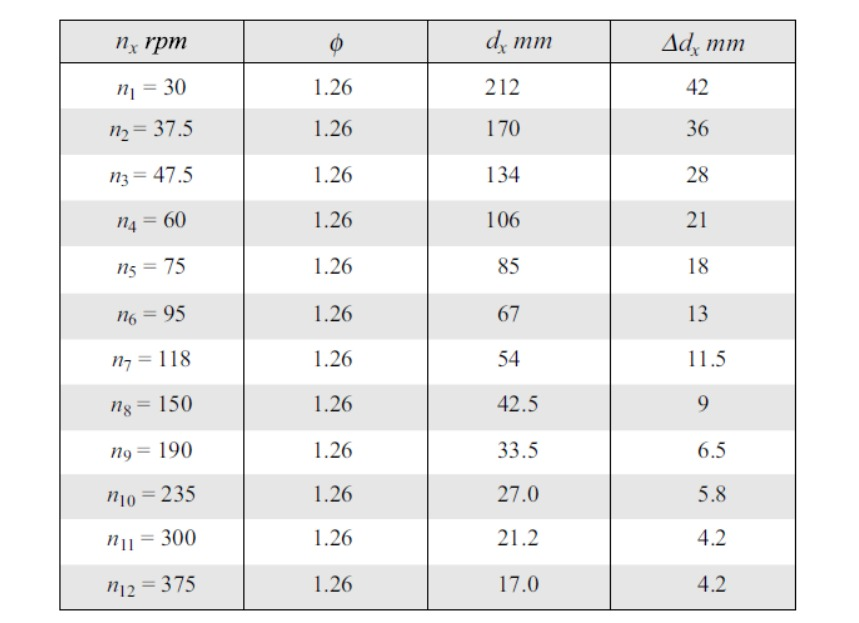
\includegraphics[width=\linewidth]{img/table_d.jpeg}
    \caption{chart for $\Delta$d}
  \end{subfigure}
  \hfill
  \begin{subfigure}{0.48\textwidth}
    \centering
    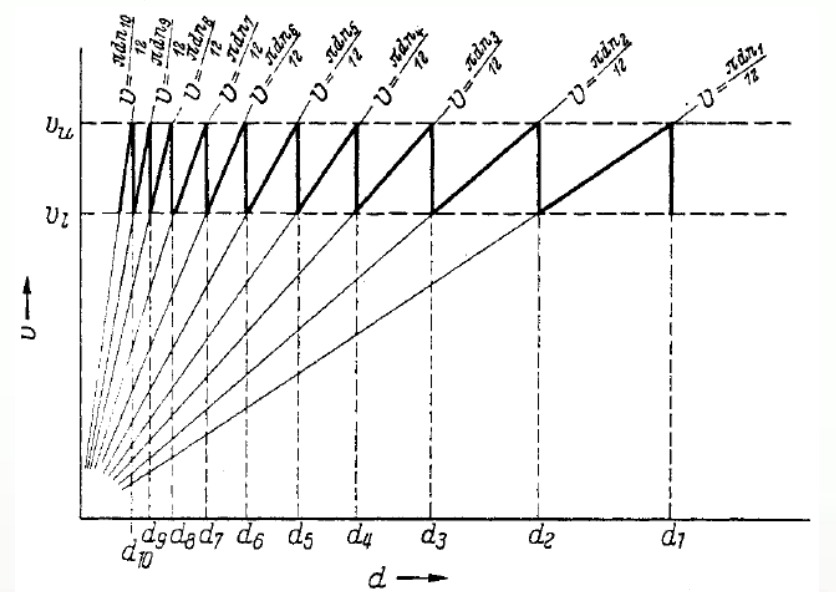
\includegraphics[width=\linewidth]{img/saw_dia.jpeg}
    \caption{saw diagram}
    \label{fig:saw diagram}
  \end{subfigure}
\end{figure}

\begin{itemize}
  \item $$\frac{n_n}{n_{n-1}} = \frac{v_u}{v_l}$$
  \item $$\phi = \frac{v_u}{v_l}$$
  \item Generally depth of cut, t is kept upto 5mm.  Here, $\Delta d_1$ = 42mm, so (d/2) = (42/2) = 21mm , that means it  will need 6 revolution. 
  \item  $\Delta d_11$ = 4.2mm, that means it  will need only 1 revolution.
  \item In order to make the machine tool performance equally feasible in the
  whole rpm range, the low rpm values should be brought still closer while
  the high rpm values can be widened a little.
  \item So, depth of cut will not be uniform in this case. To make it uniform, some extra steps are added for lower speeds, and some steps are ignored at higher speeds. So that, depth of cut will remain similar or nearby. 
\end{itemize}

\section{Lecture 4: Arithmatic Progression (AP) \& Logarithmic Progression (LP) Series}
\hfill Date: 11/07/2023

\subsection*{Arithmatic Progression (AP) series}
\begin{align*}
  n_1 \\
  n_2 &= n_1 + a \\
  n_3 &= n_2+ a = n_1 + 2a\\
  ...\\
  ...\\
  n_z &= n_1 + (z-1) a 
\end{align*}

Here, $$\phi_1 = \frac{n_1 + a}{n_1}$$
and, $$\phi_2 = \frac{n_1 + 2a}{n_1 + a}$$

So, $\phi$'s are not same in AP. 

\subsubsection*{Example}
Calculate the rpm values and diameter range served by each rpm for
the following conditions:\\
$n_1$ = 30 rpm,
$n_z$ = 375 rpm,
Number of speed steps, z = 12,
v = 20 m/min, Assume, initial diameter = 212 mm.

\textbf{Solution:}\\
$$d_x = \frac{1000 v}{\pi n_x}$$
$$d_{x+1} = \frac{1000 v}{\pi n_{x+1}}$$
so, we get,
$$\Delta d_x = \frac{1000 v}{\pi} \times \left(\frac{1}{n_x} - \frac{1}{n_{x+1}}\right) $$

\begin{figure}[h]
  \centering

  \begin{subfigure}{0.48\textwidth}
    \centering
    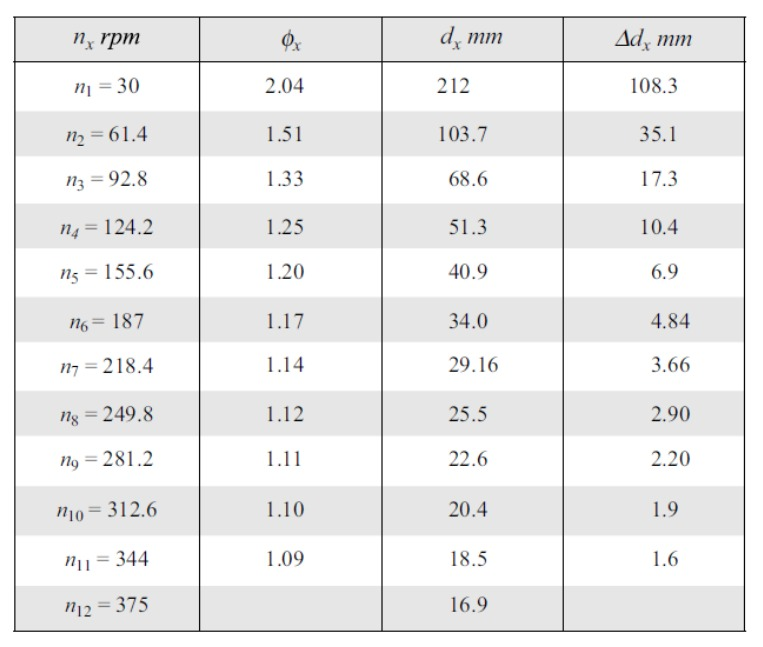
\includegraphics[width=\linewidth]{img/ap_table.jpeg}
    \caption{chart for $\Delta$d}
  \end{subfigure}
  \hfill
  \begin{subfigure}{0.48\textwidth}
    \centering
    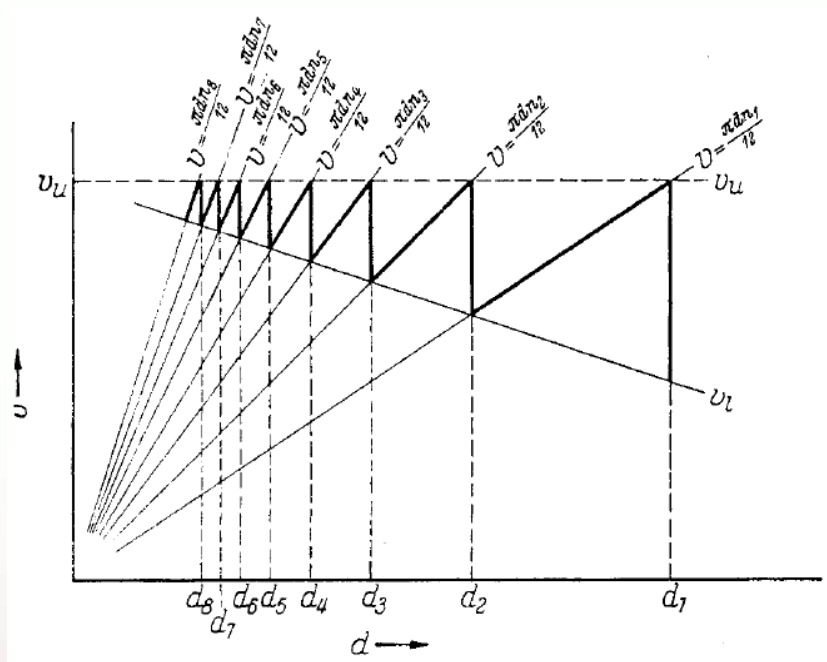
\includegraphics[width=\linewidth]{img/saw_dia_ap.jpeg}
    \caption{saw diagram}
    \label{fig:saw diagram of AP}
  \end{subfigure}
\end{figure}


\subsection*{Logarithmic Progression (LP) series}
\begin{align*}
  \Delta d_x &= 2 Md_x^p \\
  \Delta d_x &\propto d_x 
\end{align*}

Here, M and p are constant. Generally, p = 0.5. In this progression, no. of cut are nearly uniform. That's why better than previous two progression. 

Again, 
\begin{align*}
  \Delta d_x &= 2 Md_x^p \\
  d_x - d_{x+1} &= 2Md_x^p \\
  d_{x+1} &= d_x \left(1 - \frac{2M}{d_x^{1-p}}\right) \\
  \frac{1000 v}{\pi n_{x+1}} &= \frac{1000 v}{\pi n_{x}} \left(1 - \frac{2M}{\left(\frac{1000 v}{\pi n_{x}}\right)^{1-p}}\right) \\ 
  \frac{n_x}{n_{x+1}} &= 1 - 2M  \left(\frac{\pi n_{x}}{1000 v}\right)^{1-p}\\
  \frac{1}{\phi_x} &= 1 - 2M  \left(\frac{\pi n_{x}}{1000 v}\right)^{1-p}
\end{align*}

\subsubsection*{Example}
Calculate the rpm values and diameter range served by each rpm for
the following conditions:\\
$n_1$ = 30 rpm,
$n_z$ = 361 rpm,
Number of speed steps, z = 12,
v = 20 m/min, Assume, initial diameter = 212 mm.

\subsubsection*{Solution}
Here, M = 0.88 (approx.)  and p = 0.5 

\begin{figure}[h]
  \centering

  \begin{subfigure}{0.48\textwidth}
    \centering
    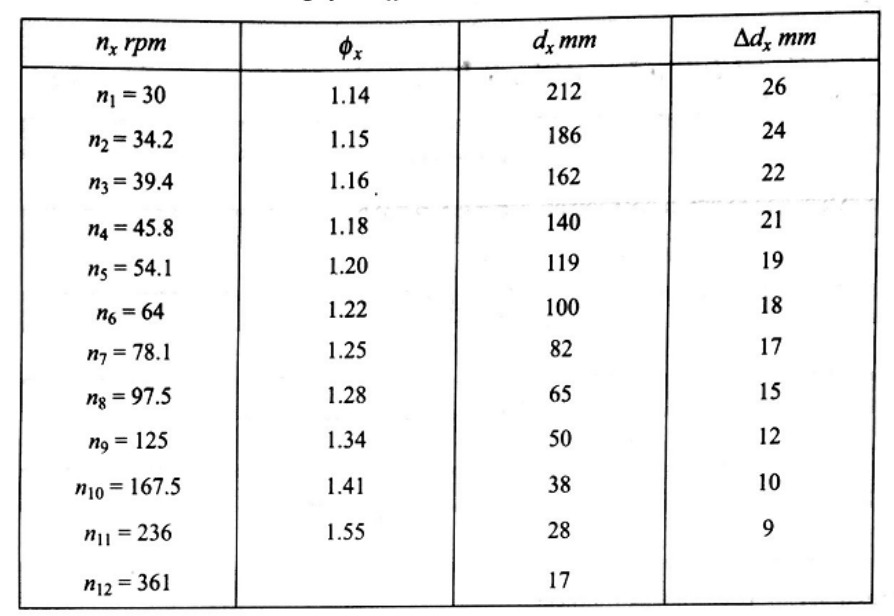
\includegraphics[width=\linewidth]{img/lp_table.jpeg}
    \caption{chart for $\Delta$d}
  \end{subfigure}
  \hfill
  \begin{subfigure}{0.48\textwidth}
    \centering
    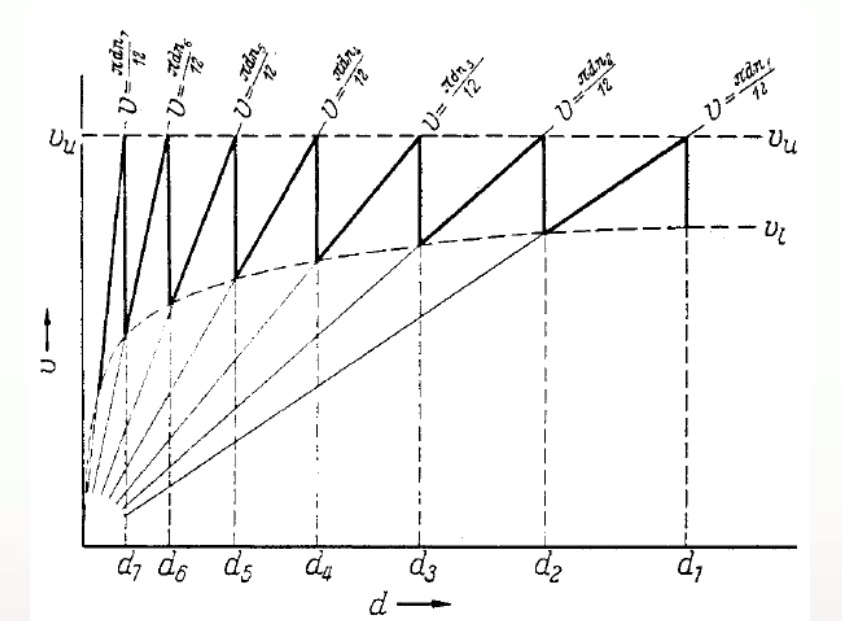
\includegraphics[width=\linewidth]{img/saw_dia_lp.jpeg}
    \caption{saw diagram}
    \label{fig:saw diagram of LP}
  \end{subfigure}
\end{figure}

\subsection*{Kinematic Advantages of Geometri Progression}

\subsubsection*{Constant loss of Economic Cutting Speed in the whole rpm range}
\begin{figure*}[h]
  \begin{center}
    \includegraphics*[width=0.95\linewidth]{img/kinematic_advantage.png}
  \end{center}
\end{figure*}

$\Delta v_j = \text{the loss of economic cutting speed} = v_{opt} - v_j$
 (lowest distance of $V_{opt}$ from either $V_j$ or $v_{j+1}$, for max $\Delta v_j$, $v_{opt}$ will be at the center)

 \begin{align*}
  \frac{\left(\Delta v_j\right)_{max}}{v_{opt}} &= \frac{\left(v_{j+1} - v_j\right)/2}{\left(v_{j+1} + v_j\right)/2} \\
  \left(\Delta v_j\right)_{max} &= \frac{\left(n_{j+1} - n_j\right)}{\left(n_{j+1} + n_j\right)} \times v_{opt} \\
  \left(\Delta v_j\right)_{max} &= \frac{\phi_{j} - 1}{\phi_{j} + 1} \times v_{opt} \\
 \end{align*}

 \subsubsection*{Constant loss of Productivity in the whole rpm range}
 The rate of material removal, $Q = 1000 \times t  \times s \times v $  $mm^3/min$. 

Now, maximum relative loss of production volume : 
$$\left(\frac{\Delta Q}{Q}\right)_{max} = \left(\frac{\Delta v}{v}\right)_{max} = \frac{n_{j+1} - n_j}{n_{j+1} } = \left(1 - \frac{1}{\phi}\right) $$ 

\subsubsection*{Better Design Features}
If number of steps are reduced to half, still the ratio remains same. 
$$n - n\phi - n\phi^2 - n\phi^3 - n\phi^4 - n\phi^5$$
$$n  - n\phi^2 - n\phi^4 $$
$$\overbrace{\phi^2} -- \overbrace{\phi^2} $$

If A times increased, still the ratio remains same. 
$$An - An\phi - An\phi^2 - An\phi^3 - An\phi^4 - An\phi^5$$
$$\overbrace{\phi} - \overbrace{\phi} - \overbrace{\phi} - \overbrace{\phi} - \overbrace{\phi}$$

If $\phi^2$ times increased, still the ratio remains same. 
$$An\phi^2 - An\phi^3 - An\phi^4 - An\phi^5$$
$$\overbrace{\phi} - \overbrace{\phi} - \overbrace{\phi} $$

$R_n = R_v \times R_d$

\subsection*{Selection of Speed Steps}
\begin{align*}
  &\Rightarrow n_z = n_1 \phi^{z-1} \\
  &\Rightarrow \phi^{z-1} = \left(\frac{n_z}{n_1}\right) = R_n \\
  &\Rightarrow (z-1) \log \phi = \log R_n \\
  &\Rightarrow z \log \phi = \log \left(R_n \phi\right) \\
  &\Rightarrow z = \frac{\log \left(R_n \phi\right)}{\log \phi} 
\end{align*}

\subsection*{Standard values of $\phi$}
$$n_x \phi^{s_1} = 2nx$$
$$n_x \phi^{s_2} = 10nx$$

\begin{align*}
  \phi &= 2^{1/s_1} = 10^{1/s_2} \\
  &\frac{1}{s_1} \log 2 = \frac{1}{s_2} \log 10 \\
  &\frac{s_2}{s_1} = \frac{\log 10}{\log 2} = \frac{1}{0.3} = \frac{10 s'}{3s'}  
\end{align*}

so, $s_2 = 10s'$ and $s_1 = 3s'$ 
\subsubsection*{IMPORTANT}
$$if \, \phi \uparrow \, , \left[\frac{\phi - 1}{\phi + 1}\right] \uparrow \, , \frac{\phi -1}{\phi} \uparrow $$ 
so, $\phi$ should be low in order to minimize losses. 

Again, $$z = \frac{\log \left(R_n \phi\right)}{\log \phi}$$
if $\phi \uparrow , z \downarrow $ and if $\phi \downarrow , z \uparrow $

so, if $\phi$ decreases, no. of speed steps increase, hence design becomes complicated and costly.

Therefore, we've to find the optimum of $\phi$. 

\begin{itemize}
  \item Let z = 6.5 found, but no. of steps can not be fractions. So, it have to be round off. While rounding off, we have to select the number which is multiple of 2 or 3. Hence, z = 6 have to be taken, and z $\neq$ 7, as it is not divisible by 2 or 3. 
\end{itemize}
\vspace*{1cm}

\section{Lecture 5: Transmission range of a group}
\hfill Date: 22/07/2023
 
\begin{multicols*}{2}
  Let, z = 12, then it have to represent in multiple of 2 and 3. so, z = $2 \times 3 \times 2$.

  $$i_{min} = \frac{1}{4} \,\,\,\, \& \,\,\,\, i_{max} = 2$$

  $$\text{Transmission Ratio, T.R.} = \frac{i_{max}}{i_{min}} = 8$$

  \subsubsection*{GP}
  $n$ - $n \phi$ - $n \phi^2$ - $n\phi^3 - n\phi^4$ \\
  $\frac{n_2}{n_1} = \phi^x$, here $x$ indicates after how many steps we got the speed. \\
  For example - \\
  $n$ - $n \phi^2$ - $n\phi^4$ \\ 
  Here, x = 2 \\

  x = characteristics of transmission rate \\

  \begin{align*}
    \text{Structural formula, S.F.: } z &= p_1 \times p_2 \times p_3 \times ... \times p_n \\
    12 &= 2 \times 2 \times 3 \\  
  \end{align*}

  Here, the possible combination: $\frac{3!}{2!} = 3$ 

  \begin{align*}
    \text{Detailed Stru. for. : } z &= p_1 (x_1) \times p_2(x_2) \times p_3 (x_3) \times ... \times p_n (x_n) \\
    12 &= 2(1) \times 3(2) \times 2(6) \\
    &\\
    x_1 &= 1 \\
    x_2 &= p_1 = 2 \\
    x_3 &= p_1p_2 = 6  
  \end{align*}

  Here, the possible combination: $\frac{3!}{2!} \times 3! = 18$ 

  \subsection*{Kinematic Arrangement}
  \begin{figure}[H]
    \begin{center}
      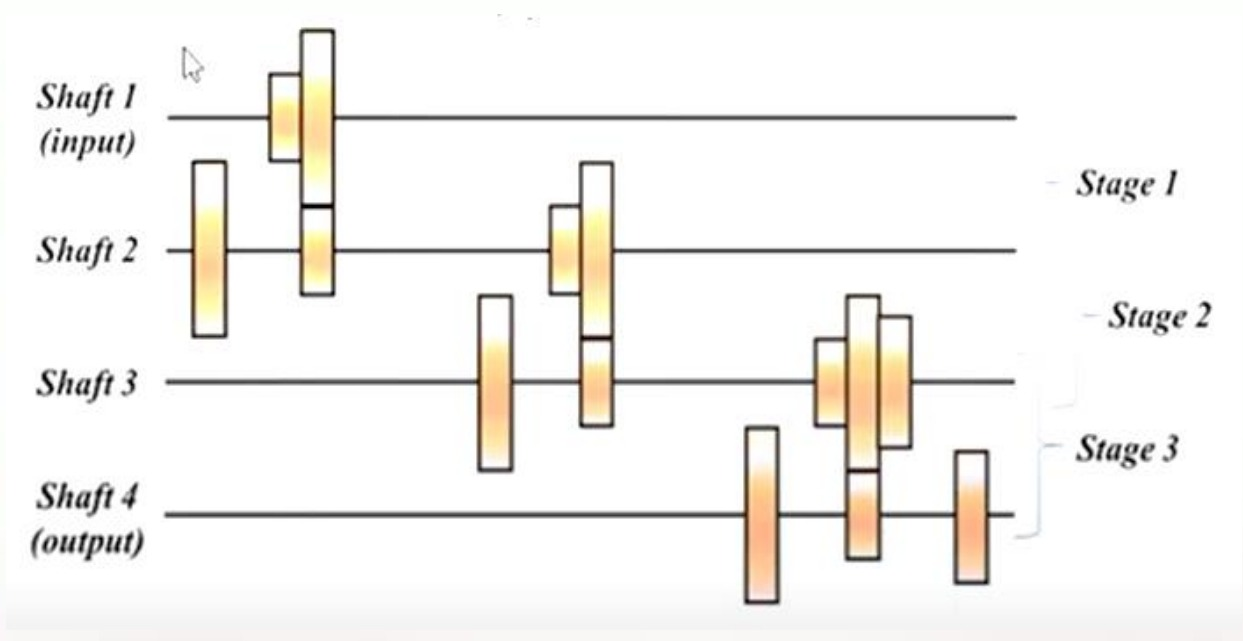
\includegraphics[width=\columnwidth]{img/kinematic_arrangement.jpeg}
    \end{center}
  \end{figure}

  \subsubsection*{Structural Diagram}
  \begin{align*}
    z &= p_1 (x_1) \times p_2(x_2) \times p_3 (x_3) \times ... \times p_n (x_n) \\
    12 &= 2(1) \times 3(2) \times 2(6) \\
  \end{align*} 

  $u = 3$ [stage] \\
  $u + 1 = 4$ [shaft] \\

  \subsubsection*{How to draw structural diagram:}
  \begin{itemize}
    \item Draw (u+1) vertical lines. 
    \item Then, draw 'z' horizontal line. 
    \item choose mid point of shaft I.
    \item Then, draw $p_1$ lines maintaining a distance of $x_1$.
    \item continue for all shafts.
  \end{itemize}

  \begin{figure}[H]
    \begin{center}
      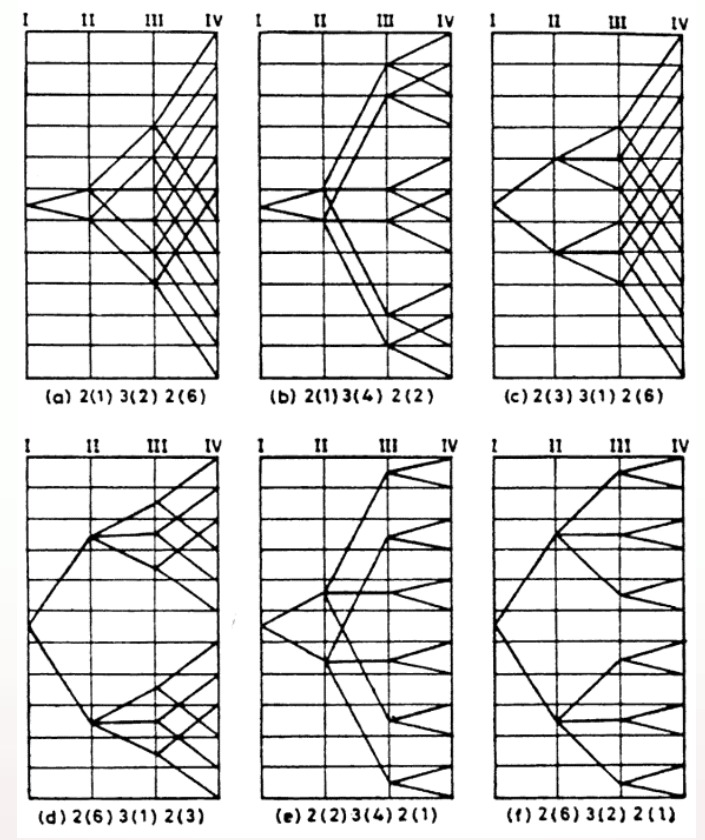
\includegraphics[width=\columnwidth]{img/structural_diagram.jpeg}
    \end{center}
  \end{figure}

  \subsubsection*{The selection of the best structural diagram}
  \begin{enumerate}
    \item $$i_g = \frac{i_{max}}{i_{min}} = 8$$
    $$i_g \leq 8$$
    \item $$\sum_{i = 1}^{u+1} d = min $$
    In the intermediate shafts, have to check which min speed has a maximum speed among them. For example - in figure, in shaft III, among the minimum speeds of all, (a) and (c) has the maximum speed. So, their diameter would be the minimum. Again, in between (a) and (c), (a) has the maximum speed of minimums at shaft II, so diameter of (a) will be the minimum.
    \item 
    \begin{align*}
      i_m &= \phi^{(p_m - 1)}x_m \\ 
      &\\
      & 2(1)\times 3(2)\times 2(6) \\ 
      &\\
      i_1 &= \phi^{(2 - 1)}1 = \phi \\ 
      i_2 &= \phi^{(3 - 1)}2 = \phi^4\\ 
      i_3 &= \phi^{(2 - 1)}6 = \phi^6\\ 
      &\\
      \phi^{x_{max}} &= \phi^6
    \end{align*}

    now, $\phi^6 < $  8, so $\phi < 1.41$ 
  \end{enumerate}

\end{multicols*}

\section{Lecture 6: Transmission of motion \& Torque}
\hfill Date: 08/08/2023

\begin{multicols}{2}
  
  \subsection*{Cone Pulley drive}
  \begin{itemize}
    \item Flat belt: Slip is more 
    \item V belt: Slip is less and effective for reducing loss 
    \item Norton gear box: When in small space we need multiple speed, then we use this.
  \end{itemize}
  
  
  \subsection*{Basic Principles for designing Sliding type claster gear}
  Let, In a triple claster gear, the number of teeth are $T_1, T_2, T_3$ respectively. 
  
  Here, $$T_2 - T_1 \geq 4$$ 

  \begin{figure}[H]
    \begin{center}
      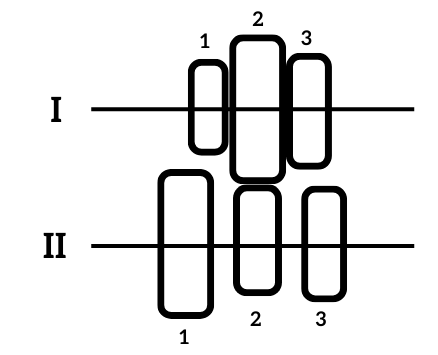
\includegraphics[width=\columnwidth]{img/claster_gear.png}
    \end{center}
  \end{figure}

  \begin{itemize}
    \item R $\rightarrow$ Addendum circle radius
    \item r $\rightarrow$ Pitch circle radius
    \item $m = \frac{d}{T}$
    \item $R = r + a = r + m$ [$\therefore a = m$]
  \end{itemize}

  \textbf{Proof:}
  \begin{align*}
    & R_{I3} + R_{II2} \leq r_{I2} + r_{II2}\\
    \Rightarrow& r_{I3} + m + r_{II2} + m \leq r_{I2} + r_{II2}\\
    \Rightarrow& r_{I3} + 2m \leq r_{I2}\\
    \Rightarrow& \frac{mT_{I3}}{2} + 2m \leq \frac{mT_{I2}}{2}\\
    \Rightarrow& T_{I3} + 4 \leq T_{I2}\\
    \Rightarrow& T_{I2} - T_{I3} \geq 4\\
  \end{align*}
\end{multicols}

\hrulefill

\end{document}
